\section{Methodology}

In the following sections, we will introduce the different hardware elements that can be instantiated on the PSoC microcontroller, and how to control these hardware elements from the microcontroller code. You will need all of these elements to solve the assigned task. Of course, the following sections are merely an introduction, not full tutorials. Small assignments will be given to learn how to use the components, but these assignments are not per se directly related to the project. Please refer to the PSoC tutorials (\url{www.cypress.com/psoc101}) or the datasheet of the hardware elements (these can be found by double-clicking on a component in the ``TopDesign.cysch'' file, and clicking on the button ``Datasheet''). 





\newpage
\subsection{General purpose input-output (GPIO)}

GPIOs are the most basic hardware elements, allowing to provide input commands to the microcontroller and receive output signals from the microcontroller. You can find tutorials of how to use GPIOs on the following website: 
\begin{itemize}
	\item \url{www.cypress.com/psoc101}, Lesson 1: ``1. Software Output Pins''
	\item \url{www.cypress.com/psoc101}, Lesson 2: ``2. Software Input Pins''
\end{itemize}
The following short assignment will help you to interface two sort of IOs~: push-buttons and LEDs. The short assignment has the following specifications: the LEDs D1-D4 must switch on when button SW1 is pushed, and switch off when this button is released. 
\begin{itemize}
	\item Locate the different peripherals present on the extension board and named in the annex \texttt{Extension\_PSoC.pdf} (LEDs, push-buttons, potentiometer, analog output connected to power amplifier, etc.). 
	\item Identify which PSoC pin number connects to each LED and each switch of the extension board. 
	\item Create a new project in PSoC creator. 
	\item In the TopDesign.cysch file, instantiate the LEDs as digital outputs (use the ``Strong Drive'' mode\footnote{this mode allows to output some current from the microcontroller, which is required to light the LEDs}). When double-clicking on a component in the TopDesign.cysch file, you open it's customized menu, where you can select the options of the component. Similarly to the video tutorial on PSoC 101, you can add the resistors, diode and ground of the extension board as off-chip component for more clarity in your design (use the schematics in the annex «Extension PSOC» for exact component values and mapping). 
	\item In the TopDesign.cysch file, instantiate the switches as digital inputs (use the ``High Impedance Digital'' mode). Again, you can add the elements of the extension board as off-chip components in your design for more clarity. 
	\item In the projectName.cydwr file, associate each LED and each switch the appropriate PSOC pin number you identified before. 
	
	\item Now go the file where you write the firmware code (i.e. main.c). You can now write the code fulfilling the specifications: 
	\begin{itemize}
		\item Locate the for(;;) loop.
        This endless loop contains the tasks that must run continuously, while the code placed before and after this loop is only executed once and is mainly used to configure the peripherals and define the variables.
		\item Write how the LEDs and switches should behave. When double-clicking on a component in the TopDesign.cysch file, you open it's customized menu. There is a button to rapidly access the datasheet of the component. Use the ``Application Programming Interface'' section to determine how to use the component from the firmware (i.e. the main.c-file). 
		\item You can use the function \texttt{CyDelay()} to put the microcontroller to sleep for a certain amount of milliseconds between two iterations of the for loop. 
		\item Build, compile and load it on the $\mu$C board, then check its behavior.
	\end{itemize}
\end{itemize}
It is important to note that, in general, microcontroller are not designed to deliver high currents. If we were using high-brightness LEDs, we would need to use \textit{buffer} circuits (such as the \texttt{74ACT244}) to provide larger currents. 






\newpage
\subsection{LCD screen}

The LCD screen is a particular output that allows you to write characters on the 16-characters LCD screen, located on the extension board. By examining the annex \texttt{Extension\_PSoC.pdf}, you will notice that the LCD requires 7 output ports from the microcontroller. On the left side of the LCD screen, there is a potentiometer that allows you to control the contrast of the LCD screen. The 8 first characters of the LCD screen are defined to be row~0, the 8 last characters of the LCD screen are defined to be row~1. The exact mapping of the rows and columns of the LCD screen are shown in Figure~\ref{fig:lcd_screen}. 
\begin{figure}[h]
	\centering
	\includegraphics[width=4in]{lcd_screen.png}
	\caption{Row and column mapping of the LCD screen. }
	\label{fig:lcd_screen}
\end{figure}
To use the LCD screen, follow the following steps: 
\begin{itemize}
	\item Instantiate a ``Character LCD" in your TopDesign.cysch file. Connect the LCD inputs to the appropriate microcontroller outputs using the ``Extension PSOC" file. 
	\item By using the API described in the datasheet of the LCD, write something on the LCD screen. The following (partial) list of functions will be particularly useful: 
	\begin{itemize}
		\item \kw{LCD\_Char\_ClearDisplay()}: to clear the LCD display; 
		\item \kw{LCD\_Char\_Position()}: to control the cursor position of the LCD display; 
		\item \kw{LCD\_Char\_PrintString()}: to print a string of characters; 
		\item \kw{LCD\_Char\_PrintNumber()}: to print the decimal value of a 16-bit value; 
		\item \kw{LCD\_Char\_PrintInt8()}: to print a two-ASCII-character hex representation of the 8-bit value; 
		\item \kw{LCD\_Char\_PrintInt16()}: to print a four-ASCII-character hex representation of the 16-bit value; 
	\end{itemize}
	Depending on which function you use to print on the LCD screen, it might be required to do a type conversion first. 
	\item Try printing some characters and some values on the LCD screen. 
\end{itemize}






\newpage
\subsection{Keyboard}

A small $4\times 3$ keyboard is provided, that can be connected directly to the bottom of the extension board\footnote{there are 8 pins to the bottom of the extension board to allow for $4\times 4$ keyboards. Please use the seven leftmost pins for a $4\times 3$ keyboard. }. Functions that allow to initialize the keyboard and to receive the pressed key are provided (i.e. the \texttt{keyboard.c} and \texttt{keyboard.h} files).  
\begin{figure}[h]
	\centering
	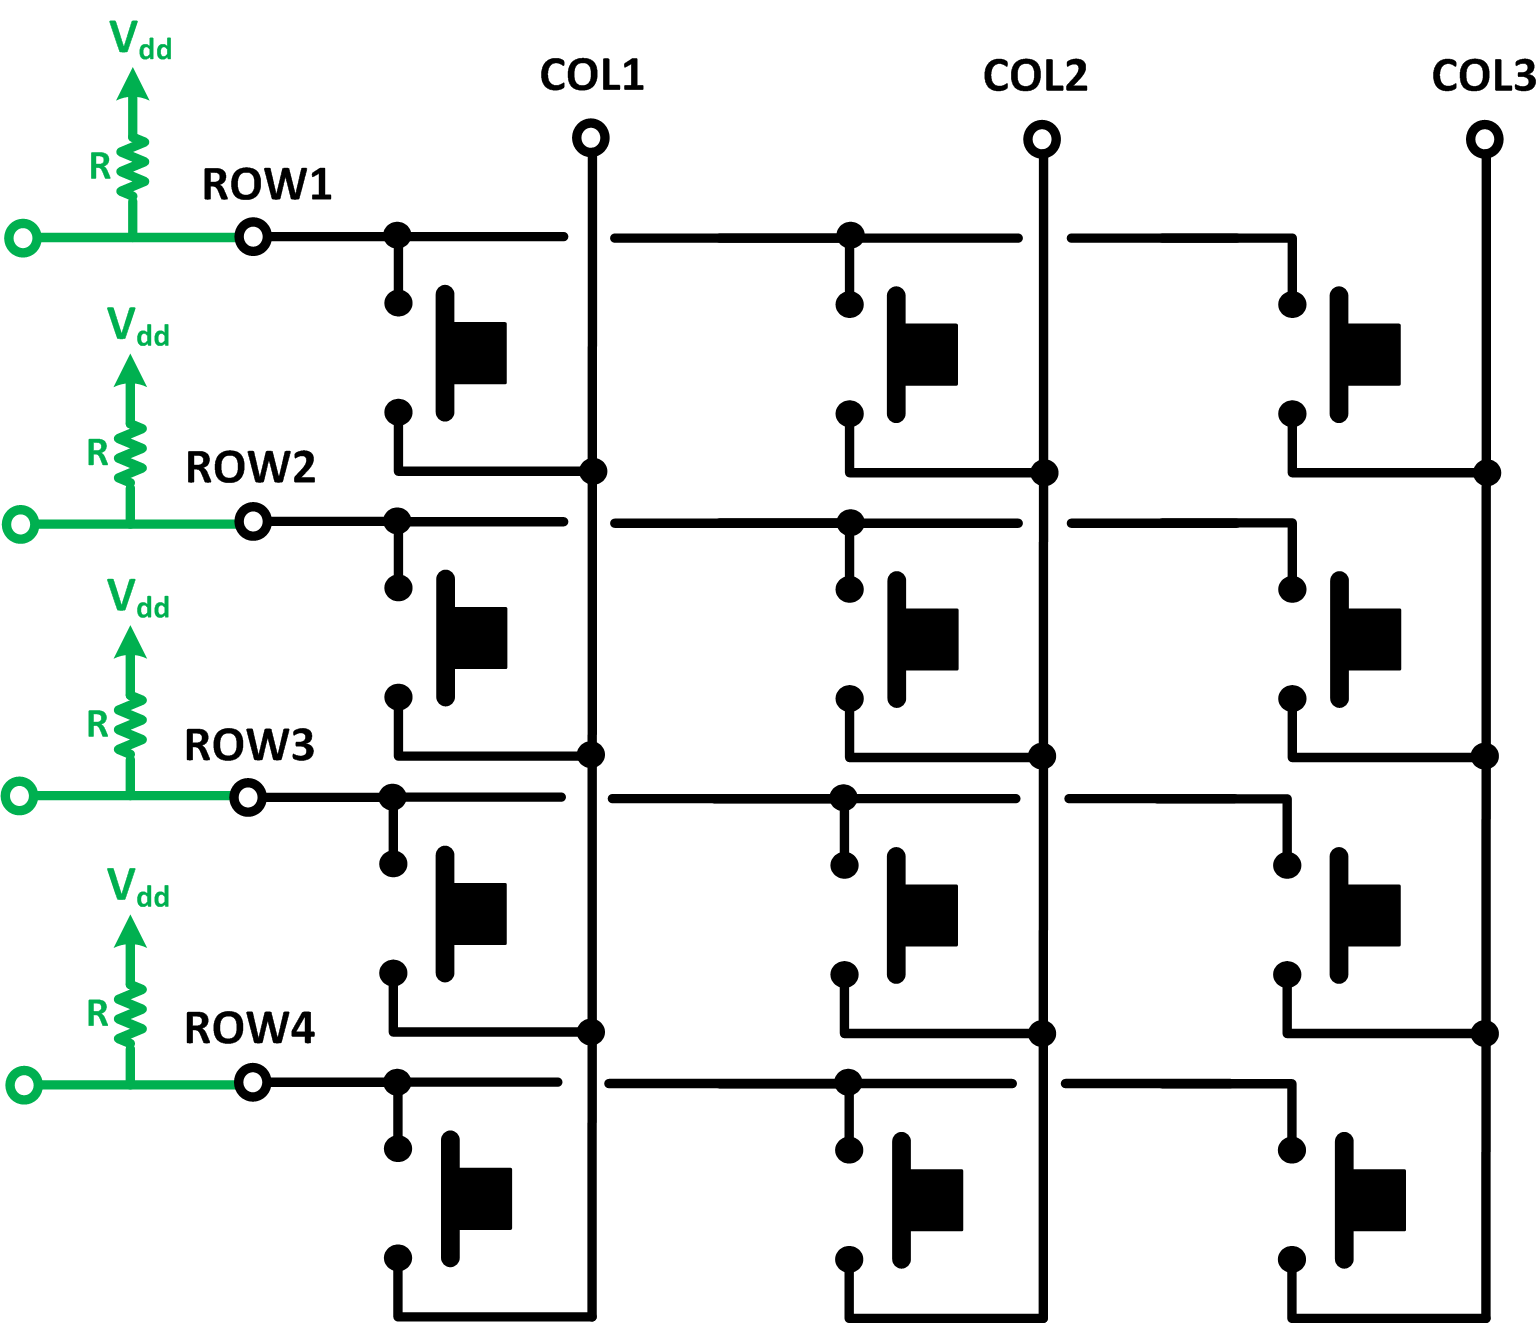
\includegraphics[width=2.5in]{keyboard.png}
	\caption{Electronic circuit of a $4\times 3$ keyboard. The green part represents the resistive pull-ups inputs of the PSoC board. }
	\label{fig:keyboard}
\end{figure}
The following short assignment will help you in using the keyboard. 
\begin{itemize}
	\item Figure~\ref{fig:keyboard} shows the electronic circuit of a matrix keyboard. Moreover, functions allowing you to read the pressed key are provided (\texttt{keyboard.c} and \texttt{keyboard.h} files). For these functions to work, the inputs ROW0, ROW1, ROW2 and ROW3 must be configured as ``Resistive pull-up'', effectively adding the green components in Figure~\ref{fig:keyboard} to the circuit. When the key is effectively pressed, the function \texttt{keypadScan()} returns the corresponding character (‘0’ to ‘9’, ‘*’ or ‘\#’).	Otherwise, it returns the value ‘z’. Using the electronic circuit of the matrix keyboard and the code provided, understand how this matrix keyboard works. 
	\item In your TopDesign.cysch file, instantiate COL0, COL1, COL2 as digital output with ``Open Drain, Drives low''. Instantiate ROW0, ROW1, ROW2 and ROW3 as Digital inputs with ``Resistive pull-up''. 
	\item Add the \texttt{keypad.h} file to the ``Header Hiles'' folder, and the \texttt{keypad.c} file to the ``Source Files'' folder. Finally, add the following line at the beginning of your firmware code (i.e. the main.c file): 
\begin{lstlisting}[style=customc]
#include "keypad.h"	
\end{lstlisting}
	\item Now write a code that prints successive pressed keys on the LCD screen. Your code should scan the keyboard every 100~ms. Note that if the keyboard is pressed only once, the value should be printed only once on the LCD screen. 
\end{itemize}






\newpage
\subsection{Analog-to-digital converter (ADC)}

Microprocessors are present in practically every industrial processes (temperature control, speed display, alarm systems) as well as in our common life (alarm-radio, audio systems, etc.). All those processes have in common the interaction with analog variables. Processors work with digital variables thus, it is necessary to convert those physical analog quantities into digital values and inversely.
\\
The transformation of physical signal to digital is done in two steps~:
\begin{enumerate}
	\item Conversion of the physical signal to measure (temperature, speed, ...) into voltage. It is the role of the sensor (thermocoupe, accelerometer, etc.).
	\item Conversion of this voltage into binary value. It is the role of the analog-to-digital converter (ADC).
\end{enumerate}
\begin{figure}[h]
	\centering
	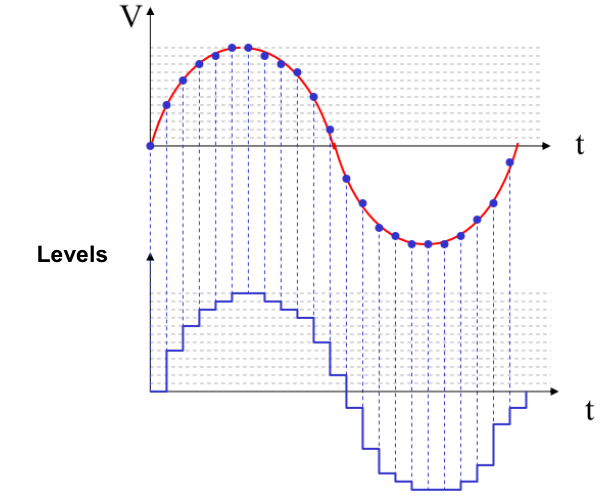
\includegraphics[width=4in]{ENdouble-quant}
	\caption{Double quantization}
	\label{fig:double-quant}
\end{figure}
The analog-to-digital converter turns an analog voltage (changing continuously) into a digital number coded on a fixed value of bits (8 to 20 bits for the PSoC).
To do so, the converter does a double quantization (see figure~\ref{fig:double-quant}): 1)~a time quantization (also called sampling), and 2)~a level quantization. Note that it is impossible to perfectly represent an analog signal into a finite number of bits.
\\
The performances of an ADC depend mostly on two parameters~:
\begin{itemize}
	\item The sampling frequency.
	\item The resolution, in other words the number N of bits coding the converted value.
    The resolution can be electrically defined as the smallest detectable change of voltage.
    If the converter has an operating range from 0~V to 5~V and convert the quantity on 10 bits, the resolution is $\frac{5 V}{2^{10}} = 4,9 mV$(\textit{i.e.} input range.
    Finally, each binary number coded on N bits will correspond to an input voltage range.
\end{itemize}


\subsubsection{Potentiometer}

In this short assignment, we will use the ADC to measure the voltage on a potentiometer connected to input \texttt{P0[7]} (see \url{Extension\_PSOC.pdf}). 
\begin{itemize}
	\item Instantiate an (analog) input pin for the signal coming from the potentiometer in the TopDesign.cysch file.
	\item Instantiate a Delta-Sigma ADC in the TopDesign.cysch file. The ADC should sample at 10~kHz with a resolution of 16 bits. Since the signal we are measuring has the same ground as the PSoC board, the ADC should be set to Single-ended mode rather than differential. Make sure to select the appropriate mode to perform a continuous ADC conversion. 
	\item Using the ADC datasheet Application Programming Interface section, determine which function you should call from the firmware (i.e. the \texttt{main.c} file) to start the ADC (this should be done in the initialization code, not in the infinite loop).  
	\item Next, determine which function you should call to start an ADC conversion. 
	\item Next, determine which function you should call to determine whether the ADC has finished it's current conversion. 
	\item Next, determine which function you should call to read the ADC value. Should you use the 16- or 32-bit version of the function? 
	\item Finally write the firmware code (i.e. the \texttt{main.c} file code) to launch an ADC conversion, check whether the ADC is finished converting, read the ADC value and write it on the LCD screen. Don't forget to start your ADC before the infinite loop! 
\end{itemize}


\subsubsection{Photoresistor}

In this project you are required to use a photoresistor to measure the luminous intensity. A photoresistor is a component whose resistance varies with luminous intensity. It has a value around 10~k$\Omega$ in the dark, and a value below 3~k$\Omega$ when the light is turned on. To use this photoresistor, you should use the electronic circuit shown in Figure~\ref{fig:meas-lum}.
\begin{figure}[h]
\center
	\begin{circuitikz}
				\draw
				(0,-2) to [phR=NSL-19M51, -o] (0,0)
				(0,-4) node [ground] {} to [R=$R_1$] (0,-2) 
				(0,0.5) node (vdd) {5V}
				(0,-2) to [short, -o] (1,-2) node (A) {}
				(0,-4) to [short, -o] (1,-4) node (B) {}
				(B) to[open, v=$V_{meas}$] (A)
				;
			\end{circuitikz}
\caption{Luminous intensity measurement with a NSL-19M51 photoresistor.}
\label{fig:meas-lum}
\end{figure}
The photoresistor is mounted on a voltage divider. The (variable) photoresistor will determine the amount of current that flows through the two resistors, hence the voltage drop over resistor $R_1$. The value of $R_1$ is 2.7~k$\Omega$ or 3.3~k$\Omega$, such that the voltage drop over $R_1$ can be measured with the PSoC ADC for all possible values of the photoresistor. If you use a single-ended ADC, don't forget to connect the ground of your circuit to the ground of your PSoC device. 
\\
In this short assignment, we will measure luminous intensity using a photoresistor. 
\begin{itemize}
	\item Use the breadboard to realize the circuit of Figure~\ref{fig:meas-lum}. The 5~V should be taken from the \texttt{POWER} pin on the PSoC device (see Figure~\ref{fig:psoc}). The ground can be connected to any ground pin of the PSoC device or extension board. 
	\item Connect the output voltage of the circuit to an (analog) input port of the PSoC device (use the GPIO inputs on the right of the extension board). 
	\item Use a Delta-Sigma ADC to measure the analog voltage. 
	\item Turn the LEDs on when the light is off, turn the LEDs off when the light is on. 
\end{itemize}




\newpage
\subsection{Timers}

A timer is a hardware element that is connected directly to the microcontroller oscillator, and is able to provide precise time management for the microcontroller. The \texttt{CyDelay()} function allows to put the microcontroller to sleep for precise time durations, but the programmer cannot know the execution time of ohter instructions. Hence, precise time managmenet is impossible to do without timers 
\\
In the following short assignment, you are asked to make the LEDs blink at a given frequency. To do so, you will need a timer. This type of peripheral has a 8/16/24/32-bits register that is decremented at each clock cycle. When the value of this register reaches 0, the counter goes back to the specified period value and starts decrementing again. At the same time, a specific bit named \texttt{TC} (in the \texttt{Timer\_Status} register) goes to 1 to warn of overflow (cf. datasheet of timer). As a first step, you will write a program allowing to make the LED blink at a frequency of 1~kHz.
\begin{itemize}
	\item Instantiate a 16-bit Timer in the TopDesign.cysch file (use the ``Fixed Function'' implementation). Set the period to cause on overflow at a frequency of 1~kHz. What is the largest period of the timer? As a reminder, the highest clock rate available in a PSoC system is a BUS\_CLK at a rate of 24~MHz.
	\item Add the launching of the timer in your program (use the Datasheet Application Programming Interface to find the appropriate function). 
	\item In the main loop of your program~:
	\begin{itemize}
		\item Check by polling if the timer has overflowed (ie. If the bit \texttt{TC} has risen to '1'). You can do so by using the following instruction: 
\begin{lstlisting}[style=customc]
overFlow = 0x80 & Timer_ReadStatusRegister(); 
\end{lstlisting}
			Explain how this instruction works? How is this line of code able to extract the bit \texttt{TC} from the \texttt{Timer\_Status} register? The datasheet mentions that the bit \texttt{TC} is ``sticky''. This means that you do not need to reset the bit \texttt{TC} to zero manually, it is reset automatically to zero after reading it.  
		\item Write a function that toggles LED4 at the overflow frequency. 
	\end{itemize}
	\item Since the human eye cannot distinguish a LED oscillating at a frequency of 1~kHz, you cannot explicitly verify if your code works well without an oscilloscope. However, you should notice that the LED does not shine as brightly as in the previous assignments. 
	\item Modify your code to obtain a period to 1~s for the blinking of the LEDs. Since a 1~s period cannot be achieved directly with a timer (see maximum period above), we rely on the code to count overflows of the timer until a 1~s period is reached. 
\end{itemize}





\newpage
\subsection{Digital-to-analog converter (DAC)}

The principle of the DAC is the opposite of the ADC~: the transformation of a number coded on N bits to a voltage in its output range.
The voltage obtained is continuous in time (the output of the converter is constant until a new conversion is done), but is always quantized because only $2^N$ different voltage values are achievable (each binary code correspond to one voltage).
\\
In the following short assignment, you are asked to realize a synthesizer capable of generating an arbitrary sound wave and convert it to sound through a speaker.
In our case, we will simply generate a sine wave at adjustable frequency~: the processor will send samples corresponding to the wanted waveform to a DAC and once rebuild, the signal will be send to the amplifier of the extension board (element U3 on the extension board). You can listen to the generated sound by connecting speakers to the audio jack. 
\begin{itemize}
	\item During the configuration of your peripherals (before the infinite loop), fill a vector (of length 100) containing the sound wave, defined as global variable so that it contains one full period of a sine wave defined between -1 and +1. To define the vector as a global variable, it needs to be declared outside of the main function. 
    To do so, you must~:
	\begin{itemize}
		\item include the file math.h in the header~;
		\item call function \texttt{sin()}, that takes as argument a floating number representing the angle (in rad) and that also returns a floating number.
	\end{itemize}
	\item Program a timer so that a sample of the sine wave is processed every 50~$\mu$s
	\item Instantiate an (analog) output pin of the DAC in the topDesign.cysch file, and connect it to the \texttt{DAC\_OUT} pin of the extension board (see \url{Extension\_ PSOC.pdf} file). 
	\item Instantiate a VDAC in the TopDesign.cysch file. The range is from 0 to 1.020~V and a slow speed is sufficient. Make sure you select ``CPU'' as the data source, since we will provide the data from the firmware (i.e. the \texttt{main.c} file). The strobe should be set to ``Register Write'', which means the DAC will provide a new analog value every time a new value is written in it's register. 
	\item In your firmware code (i.e. the \texttt{main.c} file), poll the timer to detect timer overflows (as done in the previous lab). Every 50~$\mu$s, write the next value of the sine wave vector to the DAC by using the \texttt{DAC\_SetValue()} command (that you can find in the VDAC datasheet Application Programming Interface). Note that the DAC expect to see an 8-bit signal (i.e. between 0 and 255), so you should shift (center around 128) and scale (amplitude between 0 and 128) your sine wave so that it remains within this range at all times. Don't forget to start your DAC before the infinite loop! 
\end{itemize}





\newpage
\subsection{Interrupts}

We will now study how we can use interrupts in our code to generate super-priority events. When an interrupt is latched, the firmware code in the \texttt{main.c} is temporarily interrupted while the Interrupt Service Routine (ISR) is executed. You can follow the tutorial on the following website for an introduction to interrupts: \url{www.cypress.com/psoc101}, Lesson 3: ``3. Interrupts''. 
\begin{itemize}
	\item Take your previous project on the Digital-to-Analog Converters.  
	\item To write the data to the DAC from the firmware, we will now create an Interrupt. Instantiate an Interrupt in the TopDesign.cysch file, and connect it to the interrupt-output of the timer. This means that every time the timer overflows, this interrupt will be triggered. 
	\item Following the video tutorial on interrupts, write your firmware so that your code that was previously inside your polling-loop is now in your ISR (don't forget to remove/comment out the polling of the timer). Read the documentation about the interrupt output in the timer datasheet. After an interrupt is triggered, the interrupt output remains asserted until the status register is read. To clear the status register, use the function \texttt{Timer\_ReadStatusRegister()}. 
\end{itemize}






\newpage
\subsection{Pulse Width Modulation (PWM)}

A PWM is a module that can send a square wave signal (such as shown in Figure~\ref{fig:pwm}) to a DC motor or to a servo motor. For controlling a DC motor, the ratio of high versus low state of the PWM wave determines the speed of the DC motor. For a servo motor, the length of the pulse determines the position of the servo motor. 
\begin{figure}[h]
	\centering
	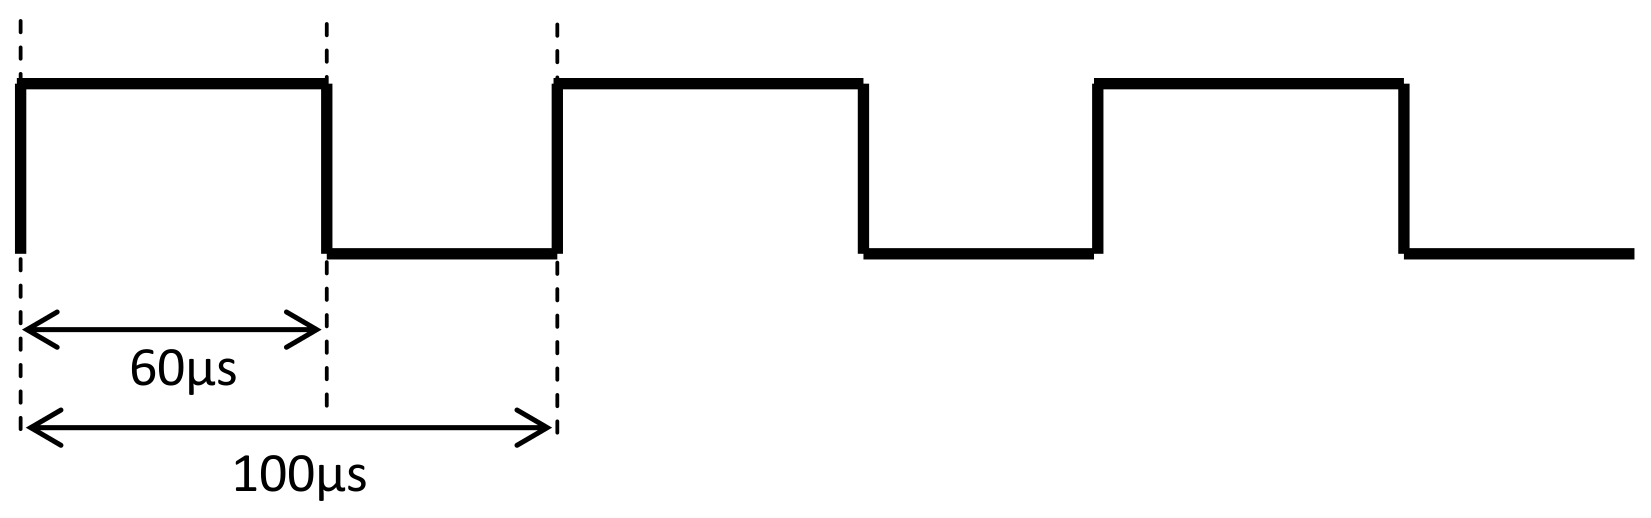
\includegraphics[width=4in]{pwm}
	\caption{PWM Signal with a duty cycle of 60 \%.}
	\label{fig:pwm}
\end{figure}
In order to use the PWM, check the tutorial on described in \url{www.cypress.com/psoc101}, Lesson 6: ``6. Pulse Width Modulator''. The principle of a PWM can be described as being a timer with two thresholds:
\begin{itemize}
	\item When the timer starts, the PWM output pin \texttt{pwm} is at ‘1’.
	\item When the counting register of the timer reaches the first threshold, named \texttt{CMP}, the output \texttt{pwm} turns to ‘0’.
	The timer continues to increment.
	\item When the counting register reaches the value of the period \texttt{Period}, the timer returns zero and the output returns to ‘1’.
\end{itemize}
By playing with the values of \texttt{CMP} and \texttt{Period}, it is possible to generate any square wave.
\\
The following short assignment will allow you to control a servo motor with a PWM module. 
\begin{itemize}
	\item Connect the servo to the microcontroller (see the servo datasheet on \url{http://www.ee.ic.ac.uk/pcheung/teaching/DE1_EE/stores/sg90_datasheet.pdf}). The orange cable should be connected to an output of J1 or J2, the black cable to the ground, and the red cable to the 5~V output pin (note that the servo consumes some current, so you cannot connect the red cable to any GPIO set to the high state). 
	\item Instantiate a PWM in the TopDesign.cysch file. The servo datasheet indicates that you need a period of 20~ms for the PWM square wave. However, by default, the maximum period of a 16-bit PWM module is 2.731~ms. To increase this range, you need to double-click on the \texttt{CLK24MHZ} block in the TopDesign.cysch. By increasing the divider value in this block, you effectively reduce the rate of the clock driving the PWM, and you increase the possible \texttt{Period} range of the PWM. Adjust the values until you reach a \texttt{Period} of 20~ms. 
	\item Adapt the \texttt{CMP} value for the pulse to have a high-value of 1.5~ms. 
	\item By using the function \texttt{PWM\_WriteCompare()}, change the duration of the pulse. What happens with a pulse of 1~ms or 2~ms? 
	\item Use the potentiometer and ADC code from the ADC assignment to make the duration of the pulse vary from 1~ms to 2~ms depending on the position of the potentiometer. 
	\item Validate that the servo is turning accordingly.
\end{itemize}







\newpage
\subsection{Serial port communications}

The serial bus allows to send and receive data from/to the microcontroller to/From the PC. This module is named UART (Universal Asynchronous Receiver / Transmitter). Before designing this communication, you will have to set the PSoC and the PC in order to make them ``speak the same language". We will start by the PSoC setup. Add an UART component to the TopDesign.cysch file. Connect the rx and the tx port of the UART component to one of the J1 or J2 GPIO ports on the PSoC extension board. Double-click on the UART component to set the UART communication parameters. The parameters of the UART connection are the following: 
\begin{itemize}
	\item Baudrate: 9600
	\item Data bits: 8
	\item No parity bit
	\item Only one stop bit
	\item No flow control
\end{itemize}

\subsubsection{Sending data to the PC}
To send and receive the data on the PC side, use a serial communications software (such as ``Termite 3.4'', that you can download on \url{https://www.compuphase.com/software_termite.htm}). This software allows to connect an USB-to-serial converter to the PC, and exchange data with an UART device. Make sure the UART communication parameters match that of the PSoC UART component. To determine the right COM port, connect the UART-to-USB converter tot he PC and do the following : 
\begin{itemize}
\item Wait for Windows to install the drivers
\item Open the Device Manager by pressing the Windows Key $+$ R. Type “devmgmt.msc” and press Enter.
\item Expand the Ports (COM \& LPT) section.
\item Find the COM port associated to the USB-to-serial (or USB-to-UART) converter. 
\end{itemize}
Connect the UART-to-USB converter between the PC and the PSoC (\textbf{note that the PSoC Tx port correspond to the UART-to-USB Rx port, and vice-versa !!!}). Do not forget to connect the ground of the PSoC to the ground of the UART-to-USB converter. 
\\
To send data to the PC from the PSoC device, refer to the UART datasheet. The following tasks need to be performed: 
\begin{itemize}
	\item Start the UART transceiver. 
	\item Test the UART transmission with the \texttt{UART\_PutString()} command
	\item Send specific data over the UART by using the \texttt{UART\_PutChar()} command. To convert an (single-digit) integer to a ASCII character, you can just add the term '0' (see code snippet below). Based on how ASCII characters are coded, can you explain why this code snippet works? 
\begin{lstlisting}[style=customc]
value_char = value_int + '0'; 
\end{lstlisting}
\end{itemize}


\subsubsection{Sending commands from the PC}

We want the PSoC to trigger an interrupt each time a byte is received from the PC on the UART port. To do this, 
\begin{itemize}
	\item Check the ``RX - on byte received'' box in the UART component in your TopDesign.cysch file
	\item add an ``Interrupt'' component connected to the \texttt{rx\_interrupt} in the TopDesign.cysch file
	\item In the firmware (i.e. \texttt{main.c} file), don't forget to start the interrupt related to the UART reception
	\item Write the code for the UART ISR, based on the sample code below. Try receiving characters from the PC and print them on the LCD. 
\end{itemize}
\begin{lstlisting}[style=customc]
CY_ISR ( isr_uart_rx_Handler ) {
    uint8_t status = 0;
    do{
        // Checks if no UART Rx errors
        status = UART_ReadRxStatus();
        if ((status & UART_RX_STS_PAR_ERROR) | 
            (status & UART_RX_STS_STOP_ERROR) | 
            (status & UART_RX_STS_BREAK) | 
            (status & UART_RX_STS_OVERRUN) ) {
            // Parity, framing, break or overrun error
            LCD_Position(1,0);
            LCD_PrintString("UART err");
        }
        // Check that rx buffer is not empty and get rx data
        if ( (status & UART_RX_STS_FIFO_NOTEMPTY) != 0){
            
            rxData = UART_ReadRxData();
            // Here comes your code, ...
            // ... what do you do with rxData ? 
        }
    }while ((status & UART_RX_STS_FIFO_NOTEMPTY) != 0);    
}
\end{lstlisting}






